\documentclass[11pt]{article}
\usepackage{tutorial-students}
\usepackage{tikz}
\usepackage{tkz-graph}

\newcommand{\fillinMCmath}[1]{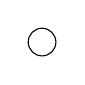
\begin{tikzpicture}\draw circle [radius=0.5em];\end{tikzpicture}\ #1}
\newcommand{\fillinMCmathsoln}[1]{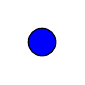
\begin{tikzpicture}\draw[black, fill=blue] circle [radius=0.5em];\end{tikzpicture}\ #1}

\newcommand{\Cats}{{\cal C}}


\author{}
\date{}
\begin{document}

\title{CPSC 320 2021W1: Assignment 4}

\maketitle
\vspace{-0.5in}

This assignment is due on \textbf{Wednesday Nov 10 at 10pm Vancouver time} on Gradescope. Assignments submitted within 24 hours after the deadline will be accepted, but a penalty of 15\% will be applied. Please follow the guidelines provided in Assignment 1.

All the submission and formatting rules for Assignment~1 apply to
this assignment as well.  For drawings of graphs, however, we will permit
pictures of hand-drawn graphs included in your PDF submission, as we did
with pseudocode on the last assignment, as long as they are clear and
easy-to-mark.

%------------------------------------------------------------------------------------
\section{List of names of group members (as listed on Canvas)}

Provide the list here. This is worth 1 mark. Include student numbers
as a secondary failsafe if you wish.

\begin{soln}
Mathew Balsdon 21041694 \\
Michael Woolsey 87234621
\end{soln}

\section{Statement on collaboration and use of resources}
To develop good practices in doing homeworks,
citing resources and acknowledging input from others, please complete the following.
This question is worth 2 marks.

\begin{enumerate}
\item All group members have read and followed the guidelines for groupwork
on assignments given on the website (see \url{https://www.students.cs.ubc.ca/~cs-320/2021S2/coursework.html}, under Assignments).
\fillinMCmathsoln{Yes} \hspace{.5in} \fillinMCmath{No}

\item We used the following resources (list books, online sources, etc. that you consulted):

\begin{soln}
none
\end{soln}

\item One or more of us consulted with course staff during office hours.

\fillinMCmath{Yes} \hspace{.5in} \fillinMCmathsoln{No}

\item One or more of us collaborated with other CPSC 320 students; none of us took
      written notes during our consultations and we took at least a half-hour break afterwards.

\fillinMCmath{Yes} \hspace{.5in} \fillinMCmathsoln{No}

      If yes, please list their name(s) here:


\item One or more of us collaborated with or consulted others outside of CPSC 320; none of us took written notes during our consultations and we took at least a half-hour break afterwards.

\fillinMCmath{Yes} \hspace{.5in} \fillinMCmathsoln{No}

      If yes, please list their name(s) here:

\end{enumerate}
\newpage

\section{ARFFH!} \label{sec:arrfh}

Heaps were covered in CPSC~221.  If you need a quick refresher,
you can check, e.g., the Wikipedia page at
\url{https://en.wikipedia.org/wiki/Heap_(data_structure)}.
Actually, whether you need a refresher or not, please take a moment
to review the Wikipedia page --- don't worry, we'll still be here
when you get back.  There's some variation in how heap operations
are presented and named, and we will use the Wikipedia article's
conventions and notation.  In particular, we will use max-heaps (where
the root has the \textit{largest} element); and the array will start with
the root at position 0, which means that the parent, left child, and
right child of node $i$ will be at positions $\lfloor (i-1)/2 \rfloor$,
$2i+1$, and $2i+2$ respectively.

A useful heap operation (called \textit{heapify} in the Wikipedia page,
or sometimes ``build heap'') is to take an array of $n$ numbers and
rearrange them into a heap.  A straightforward way to implement this
is to insert each number into the heap one at a time,
which takes worst-case $\Theta(\log i)$
time for the $i$th insertion, and gives overall worst-case $\Theta(n\log n)$
runtime for the entire heapify operation.

A better implementation is due to Bob Floyd, and is sometimes called
Floyd's Heapify.  This is usually presented iteratively:
\begin{algorithmic}[1]
\Function{FloydsHeapify}{A,n} \Comment{Converts array $A$ of size $n$ into a heap}
\For{$i=n-1$ down to $0$}
  \State sift-down(i) 
\EndFor
\EndFunction
\end{algorithmic}
where the \textit{sift-down} operation is the one where you start at
$A[i]$ and iteratively keep swapping with the larger of its two children,
moving the value that started at $A[i]$ downward in the heap until
the heap order property is established.  Sift-down can take time
proportional to the height of the heap, which is $\log n$ at the root,
so Floyd's heapify algorithm is clearly $O(n\log n)$.  However,
a more careful analysis shows that it actually runs in worst-case
time $\Theta(n)$.  This analysis (which you hopefully saw in CPSC~221)
is usually presented as a tricky summation, or there's a very slick
ammortized analysis, which you can ask us about on Piazza.

However, in \textit{this} problem, we will show how to implement
Floyd's heapify as a recursive, divide-and-conquer algorithm,
and then show how solving the corresponding runtime
recurrence gives you the same linear time bound!
Here's Alan's Recursive Reformulation of Floyd's Heapify (ARRFH):
\begin{algorithmic}[1]
\Function{ARRFH}{A,i,n}
\Statex // Makes the subtree rooted at entry $A[i]$ obey the heap order property.
\Statex // Call ARRFH(A,0,n) to convert the entire array.
\If{$i\ge n$}
  \Return \Comment{Base Case:  Past the end of the array.  Nothing here to heapify.}
\EndIf
\State ARRFH(A,2i+1,n) \Comment{Heapify left subtree.}
\State ARRFH(A,2i+2,n) \Comment{Heapify right subtree.}
\State sift-down(i) 
\EndFunction
\end{algorithmic}

\begin{enumerate}
\item (2 marks)
Prove that ARRFH is correct, i.e., prove that it establishes the
heap order property (each node's value is larger than both of its children)
throughout the heap.
You may assume that the heap is a complete, balanced binary tree, and
that the numbering scheme ($2i+1$ and $2i+2$ for the left and right
children of node $i$) is correct.
You should also rely on the correctness property of sift-down:
that if the tree rooted at node $2i+1$ obeys the heap order property,
and the tree rooted at node $2i+2$ obeys the heap order property,
then calling sift-down at node $i$ results in the tree rooted at
node $i$ obeying the heap order property.
(\textbf{Hint:}  Your proof should be extremely short and rely
on the recursive structure of the code.  It's actually an induction proof,
but I'm afraid that if I say ``induction'', a bunch of you will start
obsessing over assuming some statement for $i$ and proving for $i+1$.
It's really a structural induction, or if you insist, you can do your
induction on the height of the subtree rooted at node $i$.)

\begin{soln}
On calling this function, we call ARRFH on node $i$'s children $A[2i+1]$ and $A[2i+2]$ and then proceed to call sift-down on $i$. If $i$'s children are leaves then they already obey heap order, so $i$ will obey heap order after sifting as well by the correctness property of sift-down. If they are not leaves, we recursively call ARRFH on their children again until hitting leaves. The recursion folds, sifting down in level-order from the leaves up, meaning all nodes end up obeying heap order due to sift-down's correctness. \\
\end{soln}

\item (2 marks)
Write a recurrence relation for the worst-case runtime of ARRFH.
As before, you may assume that the heap is a complete, balanced binary tree, and
that the numbering scheme ($2i+1$ and $2i+2$ for the left and right
children of node $i$) is correct.
You may assume that the call to sift-down(i) takes worst-case
$\Theta(\log k)$ time, where $k$ is the number of nodes in the subtree
rooted at $i$.

\begin{soln}
Given a tree of size n, the worst case will be one where the tree is perfect (if it wasn't perfect we'd be doing work on less nodes). In this case, the work on a node $i$ is equal to the work needed for $i$'s left subtree, plus the work needed for $i$'s right subtree, plus the work required to sift-down($i$), which is $\log k)$ in the worst case. The work needed when $n=1$ is constant, because this implies we are working on a leaf node with no subtrees.

$T(n) = \left\{
  \begin{array}{ll}
    c_0, & \mbox{for $n < 2$}, \\
    2T(n/2) + log(n), & \mbox{for $n \ge 2$}, 
  \end{array} \right.$
\end{soln}

\item (3 marks)
If you did the preceding part very precisely, you should simplify/approximate
it so that your recurrence has the form $T(n)=aT(n/b)+f(n)$ for
some constants $a$ and $b$ and some function $f(n)$.
This will make it easy to apply the Master Theorem.

Note that there are some different statements of the Master Theorem.
For this question, you are \textbf{required} to use the formulation
presented on Worksheet~5 in class, which we repeat here (very slightly modified):
\begin{quote}
  Suppose that $T: \mathbb{N} \rightarrow \mathbb{R}_{\ge 0}$ satisfies
  \[
  T(n) = \left\{
  \begin{array}{ll}
    c_0, & \mbox{for $n < n_0$}, \\
    a T(n/b) + c_1 n^k, & \mbox{for $n \ge n_0$},
  \end{array} \right.
  \]
  where $a > 0$, $b > 1$, $c_0 > 0$, $c_1 > 0$, and $k >0$ are constants.

  \begin{itemize}
    \item
If $a > b^k$, then $T(n) = \Theta(n^{\log_b a})$.
\item
If $a = b^k$, then $T(n) = \Theta(n^k \log n)$.
\item
If $a < b^k$, then $T(n) = \Theta(n^k)$.
\end{itemize}
\end{quote}

If you did the preceding part of this problem correctly, you'll find
that your recurrence doesn't quite fit this version of the Master Theorem.
However, you can choose a value of $k$ that \textbf{upper-bounds} your
recurrence, and then apply the Master Theorem to this.
State the values of $a$, $b$, and $k$ that you choose, so that you
can apply the Master Theorem and conclude that ARRFH runs in time
$O(n)$.  You should briefly justify your answer by explaining which
case of the Master Theorem you are applying (e.g., is $a$ greater than,
equal to, or less than $b^k$, and then simplify the expressions based
on the values you chose).

\begin{soln}
Assume a function $T': \mathbb{N} \rightarrow \mathbb{R}_{\ge 0}$ satisfies:
  \[
  T'(n) = \left\{
  \begin{array}{ll}
    c_0, & \mbox{for $n < n_0$}, \\
    a T'(n/b) + c_1 n^k, & \mbox{for $n \ge n_0$},
  \end{array} \right.
  \]
Where $a=2$, $b=2$, $c_1=1$, $n_0=2$, and $k=\frac{1}{2}$. \\
Then, since $a=2>b^k=\sqrt{2}$, \\
$T'(n)=\Theta(n^{\log_2 2})=\Theta(n)$. \\

We know that $log(n) < n^\frac{1}{2}$ for all $n\in{\textbf{R}}^+$, therefore $T(n) < T'(n)$, where $T(n)$ is the recurrence relation defined in part 2 describing the work needed for ARRFH. Knowing this, and since $T'(n)=\Theta(n)$, it follows that $T(n)=O(n)$.
\end{soln}


\end{enumerate}

\newpage

\section{Bounding Craziness}

For this problem, we will continue to use the formulation of the
Master Theorem from Question~\ref{sec:arrfh} (and in Worksheet~5).
Consider this crazy recurrence relation:
  \[
  T(n) = \left\{
  \begin{array}{ll}
    1, & \mbox{for $n < n_0$}, \\
    T(n/2) + T(5n/9) + T(4n/7) + n^2, & \mbox{for $n \ge n_0$},
  \end{array} \right.
  \]
Unfortunately, the Master Theorem doesn't apply directly to this
recurrence, and expanding out the recursion tree looks very painful!
However, there are still ways to solve (or at least bound) this
recurrence!

\begin{enumerate}
\item (2 marks)
Consider this nicer recurrence relation:
  \[
  L(n) = \left\{
  \begin{array}{ll}
    1, & \mbox{for $n < n_0$}, \\
    L(n/2) + L(n/2) + L(n/2) + n^2, & \mbox{for $n \ge n_0$},
  \end{array} \right.
  \]
Fortunately, the Master Theorem does apply to this recurrence!
What are the values of $a$, $b$, and $k$, and what does the
Master Theorem give as the big-$\Theta$ bound for $L(n)$?

\begin{soln}
$L(n) = \left\{
  \begin{array}{ll}
    1, & \mbox{for $n < n_0$}, \\
    3L(n/2) + n^2, & \mbox{for $n \ge n_0$}, 
  \end{array} \right.$ \\
  $a=3, b=2, k=2$,\\
  $a < b^k$ since $3 < 2^2$, so therefore $L(n) = \Theta(n^2)$
\end{soln}

\item (2 marks)
Prove that $L(n)\le T(n)$ for all $n>0$.  You may assume that $n_0$
is whatever is convenient so that your base cases work out.
You may also assume that both $L(n)$ and $T(n)$ are monotonically
non-decreasing, e.g., for all $m<n$, you have $L(m)\le L(n)$
and $T(m)\le T(n)$.
(Hint:  This should be a very short strong induction proof.)

\begin{soln}
Assume that in $L(n)$ and $T(n)$, $n_0 = 2$.

For $0>n>2$: $L(n) = 1$ and $T(n) = 1$, therefore $L(n) \leq T(n)$ for $0<n<2$.

Assume $L(n)$ and $T(n)$ are monotonically non-decreasing, and assume now that $n \geq 2$. We will compare  of the three recursive terms in $L(n)$ and $T(n)$ to each other:

$\frac{n}{2} \leq \frac{n}{2}$, therefore $L(\frac{n}{2}) \leq T(\frac{n}{2})$. \\
$\frac{n}{2} \leq \frac{5n}{9}$, therefore $L(\frac{n}{2}) \leq T(\frac{5n}{9})$. \\
$\frac{n}{2} \leq \frac{4n}{7}$, therefore $L(\frac{n}{2}) \leq T(\frac{4n}{7})$.

Since all individual terms of $L(n)$ are greater than all individual terms of $G(n)$, and since both functions add their terms, it follows that $L(n) \leq T(n)$, for all $n \geq 2$, and including the base case, we proved that $L(n) \leq T(n)$, for all $n > 0$.
\end{soln}

\item (2 marks)
Similarly, define a recurrence relation
$U(n)$ such that $T(n)\leq U(n)$ for all $n>0$, and
where you can directly solve $U(n)$ via the Master Theorem.
You should try to make $U(n)$ as tight to $T(n)$ as possible.

\begin{soln}

  $(n) = \left\{
  \begin{array}{ll}
    1, & \mbox{for $n < n_0$}, \\
    L(4n/7) + L(4n/7) + L(4n/7) + n^2, & \mbox{for $n \ge n_0$},
  \end{array} \right.$

\end{soln}


\item (2 marks)
Prove that $T(n)\leq U(n)$ for all $n>0$.  (Your proof should
be very similar to the proof you did for $L(n)$.)

\begin{soln}
Assume that in $T(n)$ and $U(n)$, $n_0 = 2$.

For $0>n>2$: $T(n) = 1$ and $U(n) = 1$, therefore $T(n) \leq U(n)$ for $0<n<2$.

Assume $T(n)$ and $U(n)$ are monotonically non-decreasing, and assume now that $n \geq 2$. We will compare  of the three recursive terms in $T(n)$ and $U(n)$ to each other:

$\frac{4n}{7} \geq \frac{n}{2}$, therefore $U(\frac{4n}{7}) \geq T(\frac{n}{2})$. \\
$\frac{4n}{7} \geq \frac{5n}{9}$, therefore $U(\frac{4n}{7}) \geq T(\frac{5n}{9})$. \\
$\frac{4n}{7} \geq \frac{4n}{7}$, therefore $U(\frac{4n}{7}) \geq T(\frac{4n}{7})$.

Since all individual terms of $U(n)$ are greater than all individual terms of $T(n)$, and since both functions add their terms, it follows that $U(n) \geq T(n)$, for all $n \geq 2$, and including the base case, we proved that $U(n) \geq T(n)$, for all $n > 0$.
\end{soln}

\item (2 marks)
What are the values for $a$, $b$, and $k$ for your $U(n)$, and
what is the resulting big-$\Theta$ bound for $U(n)$ that the
Master Theorem gives you?
(Hint:  You'll probably want a calculator to do some arithmetic with
$1/2$, $5/9$, and $4/7$, their reciprocals, and their squares...)

\begin{soln}
$a=3, b=7/4, k=2$ \\
$3 = a < b^k = (7/4)^2 = 3.0625 \implies U(n) \in \Theta(n^2)$
\end{soln}

\item (1 mark)
What big-$\Theta$ bound can you conclude for $T(n)$?

\begin{soln}
Since $L(n) \leq T(n) \leq U(n)$, and we know the bounds on $L(n)$ and $U(n)$ to be both $\Theta(n^2)$, it is true that $\Theta(n^2) \leq T(n) \leq \Theta(n^2)$, therefore it must be that $T(n)=\Theta(n^2)$.
\end{soln}

\end{enumerate}


\newpage

\section{Who's the boss?}
The start to problem is covered in Tutorial~6. The problem is
repeated here and there are two more parts to work on.

        Recently, Hooli Inc, a large international company, had an election to choose their CEO for the next 5-year period. A candidate can be selected as the new CEO, only if they gather a majority vote, meaning that from the $n$ votes submitted by shareholders, they get more than $n/2$ votes. Hooli claimed that in the recent vote no candidate got a majority, so the current CEO will be hired for the time being. A freedom of information request was made by a news agency to Hooli to disclose the votes for the election.

        Hooli said that, due to privacy concerns, they cannot disclose the votes because the reputation of the candidates with very few votes will be damaged. Instead, they have been able to quickly set up an \href{https://www.howtogeek.com/343877/what-is-an-api/}{\color{blue} \textit{API}} for the news agency. Every query to the API is
        of the form $QueryAPI(i,j)$, where $i$ and $j$ are two integers in the range $[1..n]$ (the number of votes, $n$ is known publicly). The query returns True if the $i$th vote and the $j$th vote were cast for the same candidate, and False otherwise.

As an example of how to access the API, we can run $QueryAPI(1,k)$ $n-1$ times with $k=2,\dots,n$ to count how many of the votes are given to the same candidate as the first vote. Hooli is charging a ridiculous amount of money for every query made to the API. We are interested in checking whether there is a majority in the $n$ votes or not, and we want to use the least number of queries.

\begin{enumerate}
\item \label{Hooli-give-algorithm}
(4 marks)
  Using the claim that you established in the tutorial, describe a divide-and-conquer algorithm to check whether or not some candidate has a majority, using $O(n\log n)$ queries to the API. 

\begin{soln}
The claim we have is that if candidate $x$ has a majority in list $S$, then at least one of $S_r$ and $S_l$ have a majority of $x$, where $S_r $ and $ S_l$ are each half the size of S, and are disjoint. By contraposition and De Morgan's law, we also know that if neither of $S_r $ and $ S_l$ have a majority, $S$ will not have a majority.

Starting from a list of numbers to represent the votes cast $S = \{1,2,3,...,n-1,n\}$, we will split this list into $S_l$ which is the elements from positions 1 to $\lfloor \frac{n}{2} \rfloor$, $S_r$ which is the elements from positions $\lfloor \frac{n}{2} \rfloor + 1$ to n. 

We will perform recursive calls on $S_l$ and $S_r$, all the way until we get to a base case, where the lengths of $S_l$ and $S_r$ are either 1 or 2. If the length is 1, we return S[1] (it is a majority since the group only contains itself). If the length is 2 (so we have $S_{l} $ or $ S_r = \{ i, j \}$), we will compare the two elements with an API call QueryAPI(i, j), and return either element if the call is True, otherwise return -1.

We need to merge $S_l$ and $S_r$ and check if their majority candidates keep majorities in the merged list $S$. We do this by calling QueryAPI on the majority candidate from $S_l$ on every candidate of $S$ (if a majority candidate exists), and likewise for the majority candidate from $S_r$. If such a candidate keeps a majority then we return the candidate, otherwise we return -1 to indicate there is no majority in $S$.

If at the very end we have -1, no majority exists, otherwise a majority exists for the element that was returned.
\\
\\
Please look at our code on the next page it took a while to make :-)
\newpage

\begin{algorithmic}[1]
\Function{$isMajority$}{$S[1..n]$} 
\State $\triangleright$ Returns the index of the majority element if one exists in S
\State $\triangleright$ Returns -1 if no such majority element exists in S
\State $mid = \lfloor\frac{n}{2}\rfloor$
\If{S length is 1} \Comment{Base case clause 1}
\State return $S[1] $
\ElsIf{S length is 2} \Comment{Base case clause 2}
\If{QueryAPI(S[1], S[2]) == True}
    \State return S[1] \Comment{We can return either one here}
    \Else
        \State return -1 \Comment{No majority}
    \EndIf
\Else
\State index1 = $isMajority(S[1..mid ])$ \Comment{Gets the index of the majority vote from $S_l$}
\State index2 = $isMajority(S[mid  + 1 ..n])$\Comment{Gets the index of the majority vote from $S_r$}
\State return mergeMajorities(S[1..n], index1, index2) \Comment{helper function for readability}

\EndIf
\EndFunction
\\
\Function{mergeMajorities}{S[1..n], index1, index2}
\State $\triangleright$ Helper function, combines $S_l$, $S_r$ together to return an index of S of a majority element
\State $\triangleright$ Returns -1 if no majority element exists
\If{index1 == index2 == -1} \Comment{no majority element in either $S_l$ or $ S_r$}
    \State return -1
\ElsIf{index1 == -1 XOR index2 == -1} \Comment{only 1 maj. element in $S_l$ and $ S_r$}
    \State index = whichever index is not -1
    \State votes = 1
    \For{each element i in $S[1..n]$}
        \State increment votes if QueryAPI(index, i) == True
    \EndFor
    \If{votes > mid}
    \State return index
    \Else
    \State return -1
    \EndIf
\Else
    \State votes1 = 1
    \State votes2 = 1
    \For{each element i in $S[1..n]$}
        \State increment votes1 if QueryAPI(index1, i) == True
        \State increment votes2 if QueryAPI(index22, i) == True
    \EndFor
    \If{votes1 > mid}
    \State return index1
    \ElsIf{votes2 > mid}
    \State return index2
    \Else
    \State return -1
\EndIf
\EndFunction
\end{algorithmic}

\end{soln}

\newpage

\item
(3 marks)
  Write the recurrence relation for the number of API calls, $Q(n)$, of your algorithm in part \ref{Hooli-give-algorithm}. Give a big-O bound on the number of API calls, $Q(n)$. (Hopefully it is $O(n\log n)$!)

\begin{soln}
Our base case (lines 5-11) calls $QueryAPI$ at most 1 time based on the length of $S$.

There are 2 recursive calls (lines 13, 14) to $isMajority$, both on half of the input list $S$, meaning $2Q(\frac{n}{2})$ calls.

Our "merge operation" (the function mergeMajorities) runs a for-loop $n$ times, which calls $QueryAPI$ either 1 or 2 times on each pass, therefore we have $cn$ more $QueryAPI$ calls.

Ultimately, our reccurence relation for $Q(n)$ is as such:

  $Q(n) = \left\{
  \begin{array}{ll}
    1, & \mbox{for $n < 3$}, \\
    2Q(n/2) + cn, & \mbox{for $n \ge 3$},
  \end{array} \right.$

Applying the master theorem with $a=2, b=2, k=1$, we get: \\
    $(2=2^1) \equiv (a=b^k) \implies Q(n) = \Theta(nlogn)$

\end{soln}

\end{enumerate}

\end{document}

